\section{问题二：基于离散制氨调节的运行优化}

\subsection{模型建立}

问题二将制氨产能扩至72吨/日，设备功率按扩容倍数$k=2$线性提升：碱性电解槽20~MW、质子交换膜电解槽20~MW、合成氨装置1.5~MW，制氢氨总负荷$P_{\text{H2NH3}} = 41.5$~MW，产氨能力3.0吨/h。制氨产量从72吨/日按9吨递减至36吨/日，对应运行小时数$h = Q_{\text{NH3}} / 3.0$从24小时递减至12小时。求解流程如图\ref{fig:flow_q2}所示。

\begin{figure}[H]
\centering
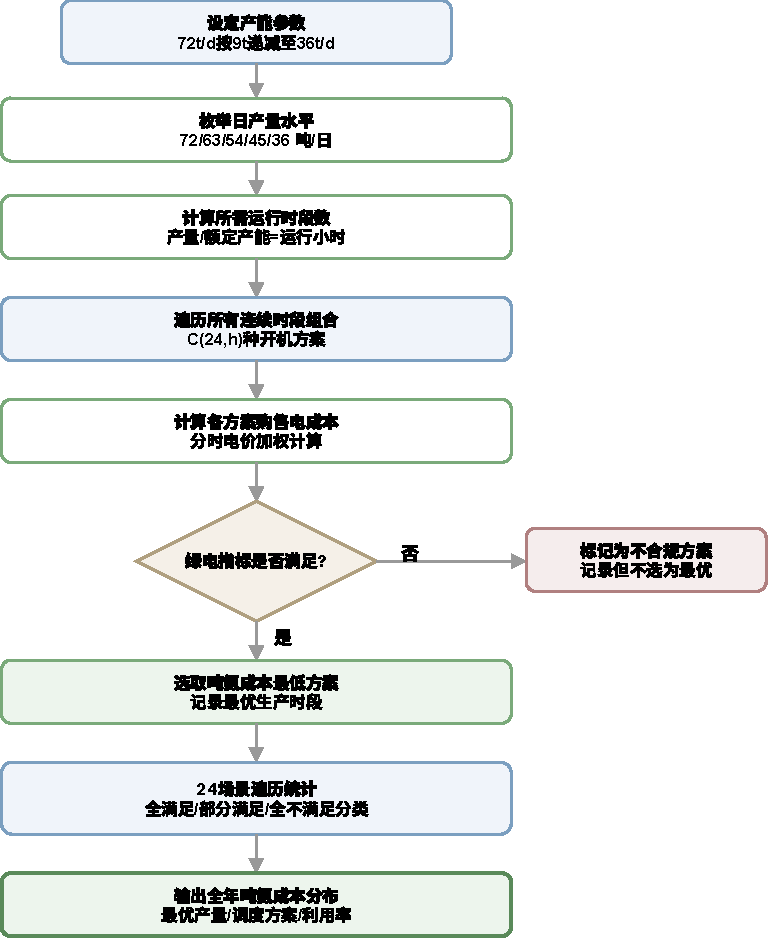
\includegraphics[width=0.85\textwidth,height=0.38\textheight,keepaspectratio]{../figures/fig_flow_q2.pdf}
\caption{问题二求解流程图}\label{fig:flow_q2}
\end{figure}

由于电氢氨装置仅有全额开机和停机两种方式，引入二进制决策变量$x(t) \in \{0, 1\}$表示时段$t$的开停机状态。优化模型如下：

\textbf{目标函数}：最小化吨氨成本
\begin{equation}
\min_{x} \quad C_{\text{ton}} = \frac{\sum_{t=1}^{24} [\lambda_{\text{buy}}(t) \cdot P_{\text{buy}}(t) - \lambda_{\text{sell}} \cdot P_{\text{sell}}(t)] \times 1000 + C_{\text{RE}} + C_{\text{OM}} + C_{\text{dep}}}{Q_{\text{NH3}}}
\end{equation}

\textbf{约束条件}：

运行时段约束：$\sum_{t=1}^{24} x(t) = h$

功率平衡约束（逐时段）：
\begin{equation}
P_{\text{net}}(t) = P_{\text{wind}}(t) + P_{\text{pv}}(t) - P_{\text{load}}(t) - x(t) \cdot P_{\text{H2NH3}}
\end{equation}
\begin{equation}
P_{\text{sell}}(t) = \max(P_{\text{net}}(t), 0), \quad P_{\text{buy}}(t) = \max(-P_{\text{net}}(t), 0)
\end{equation}

\subsection{求解算法}

由于每时段的开机决策对目标函数的贡献可以独立计算，定义时段$t$的开机边际净成本为：
\begin{equation}
\Delta C(t) = \lambda_{\text{buy}}(t) \cdot \max(P_{\text{H2NH3}} - P_{\text{surplus}}(t), 0) \times 1000 - \lambda_{\text{sell}} \cdot \max(P_{\text{surplus}}(t) - P_{\text{H2NH3}}, 0) \times 1000
\end{equation}

其中$P_{\text{surplus}}(t) = P_{\text{wind}}(t) + P_{\text{pv}}(t) - P_{\text{load}}(t)$为扣除常规负荷后的可用新能源功率。贪心策略按$\Delta C(t)$从小到大排序，选取前$h$个时段开机，该策略等价于整数线性规划的精确最优解，因为目标函数可分解为各时段独立贡献之和。

\subsection{典型场景计算结果}

\subsubsection{各产量最优方案}

在典型风光场景下，对5种产量分别求解最优开机时段安排，结果如表\ref{tab:q2_typical}所示。

\begin{table}[H]
\centering
\caption{典型场景各产量最优方案}\label{tab:q2_typical}
\begin{tabular}{ccccccc}
\toprule
产量(吨/日) & 运行时段(h) & $r_1$(\%) & $r_2$(\%) & $r_3$(\%) & 合规情况 & 吨氨成本(元/吨) \\
\midrule
72 & 24 & 86.5 & 53.3 & 6.7 & 全满足 & 6264.80 \\
63 & 21 & 84.3 & 59.7 & 7.8 & 全满足 & 5380.25 \\
54 & 18 & 80.2 & 67.3 & 9.9 & 全满足 & 4652.16 \\
45 & 15 & 51.0 & 66.7 & 24.5 & 部分满足 & 4017.60 \\
36 & 12 & 10.5 & 59.7 & 44.8 & 部分满足 & 3283.00 \\
\bottomrule
\end{tabular}
\end{table}

不同产量下的最优开机时段安排如图\ref{fig:q2_gantt}所示。产量为72吨/日时必须全天24小时运行，无优化空间；随着产量降低，优化器倾向于选择风光出力充足的白天时段开机，避开需要大量购电的夜间时段。

\begin{figure}[H]
\centering
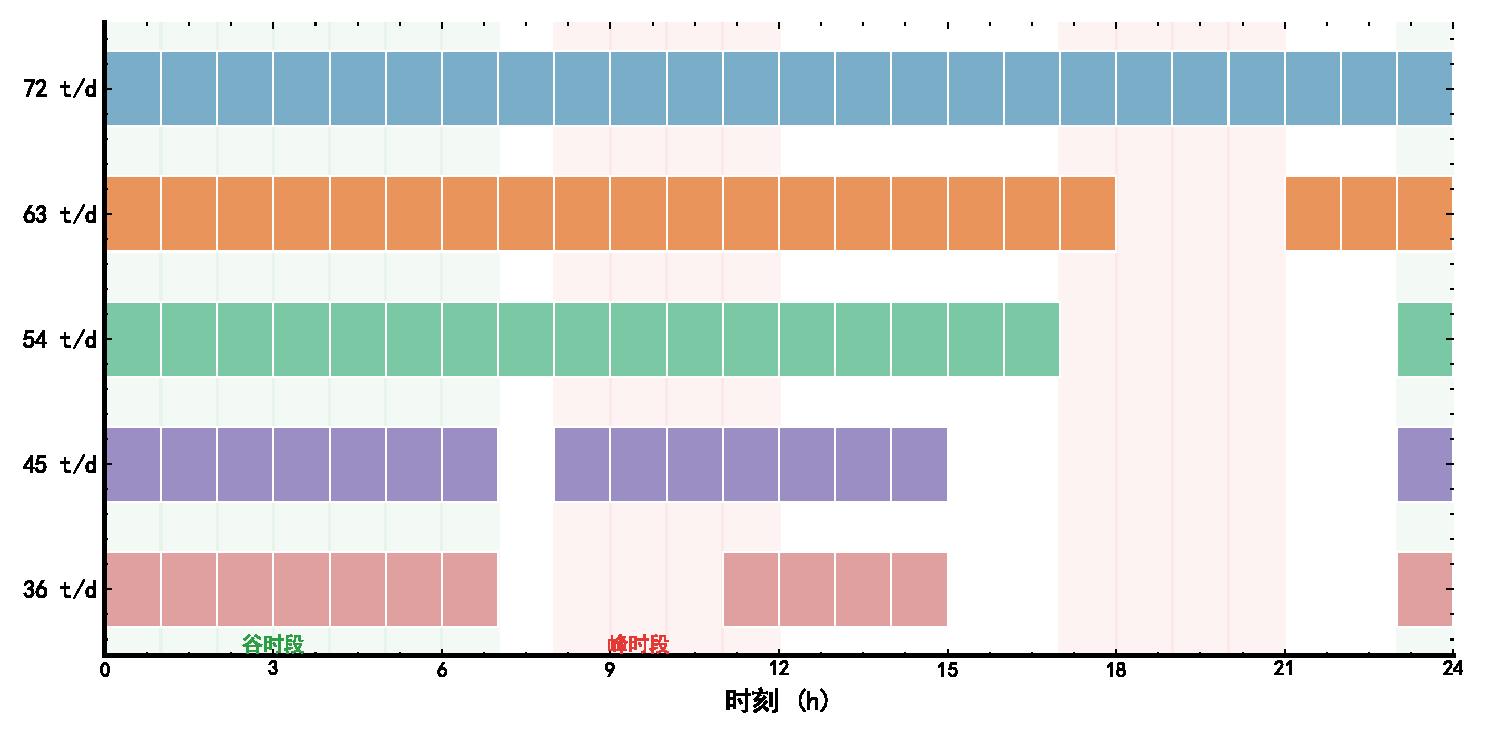
\includegraphics[width=0.92\textwidth]{../figures/fig_q2_gantt.pdf}
\caption{不同产量下最优开机时段安排甘特图}\label{fig:q2_gantt}
\end{figure}

吨氨成本随日产量的变化趋势如图\ref{fig:q2_cost_vs_production}所示。成本随产量降低而单调递减，最低吨氨成本为3283.00元/吨（产量36吨/日），但此时绿电指标仅部分满足。绿电指标全满足的最低成本方案为产量54吨/日，吨氨成本4652.16元/吨，设备利用率75\%。

\begin{figure}[H]
\centering
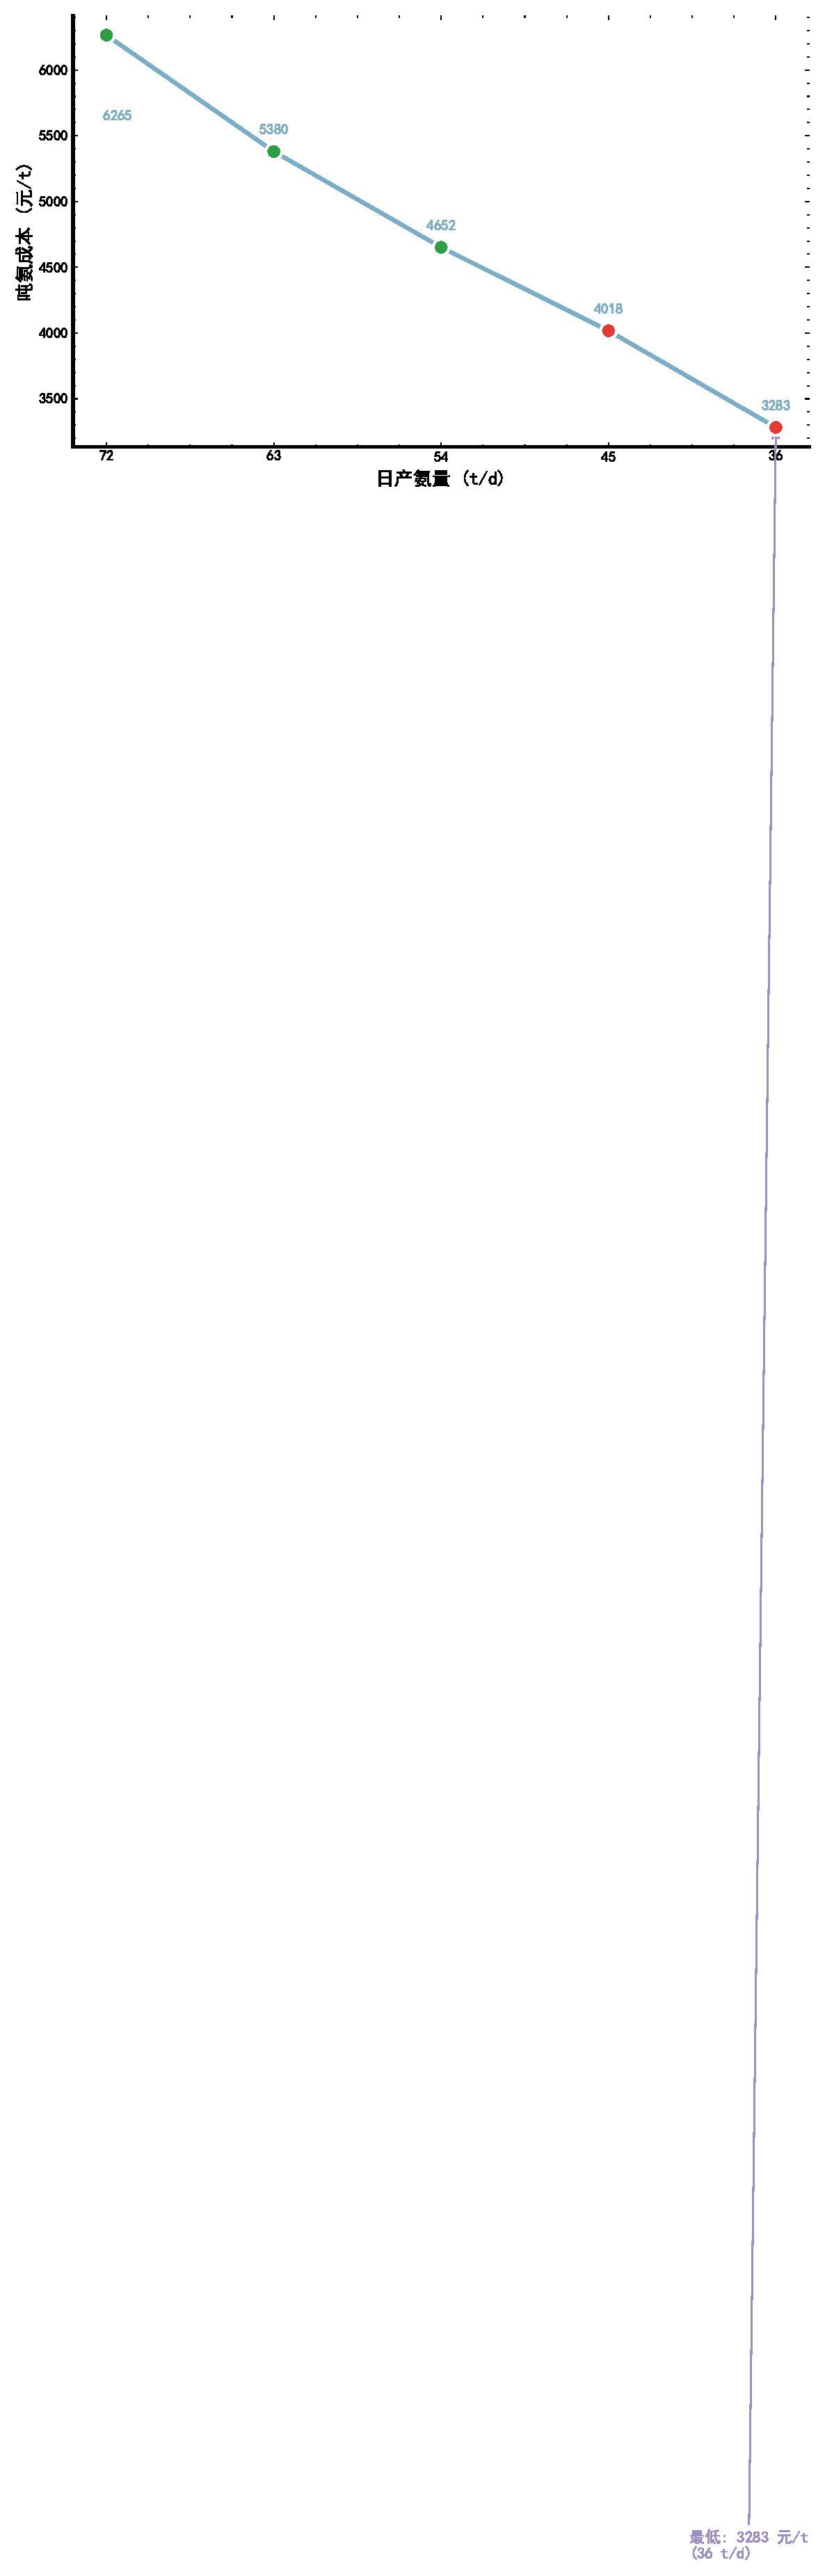
\includegraphics[width=0.85\textwidth]{../figures/fig_q2_cost_vs_production.pdf}
\caption{吨氨成本随日产量变化曲线}\label{fig:q2_cost_vs_production}
\end{figure}

产量降低导致绿电指标恶化的机制在于：运行时段减少后，开机集中在白天风光高峰期，虽然降低了购电成本，但大量夜间和傍晚的风电无法被消纳而上网，使得$r_3$（上网比例）急剧升高，$r_1$（自发自用比例）急剧降低。产量45吨/日时$r_3 = 24.5\%$已超过20\%上限，产量36吨/日时$r_3$进一步恶化至44.8\%。

\subsection{24种场景全年分析}

\subsubsection{各产量成本分布}

在24种风光组合场景（6种风电$\times$4种光伏）下，对每种产量分别求解最优方案。各产量下吨氨成本的分布情况如图\ref{fig:q2_24scenes_cost}所示。

\begin{figure}[H]
\centering
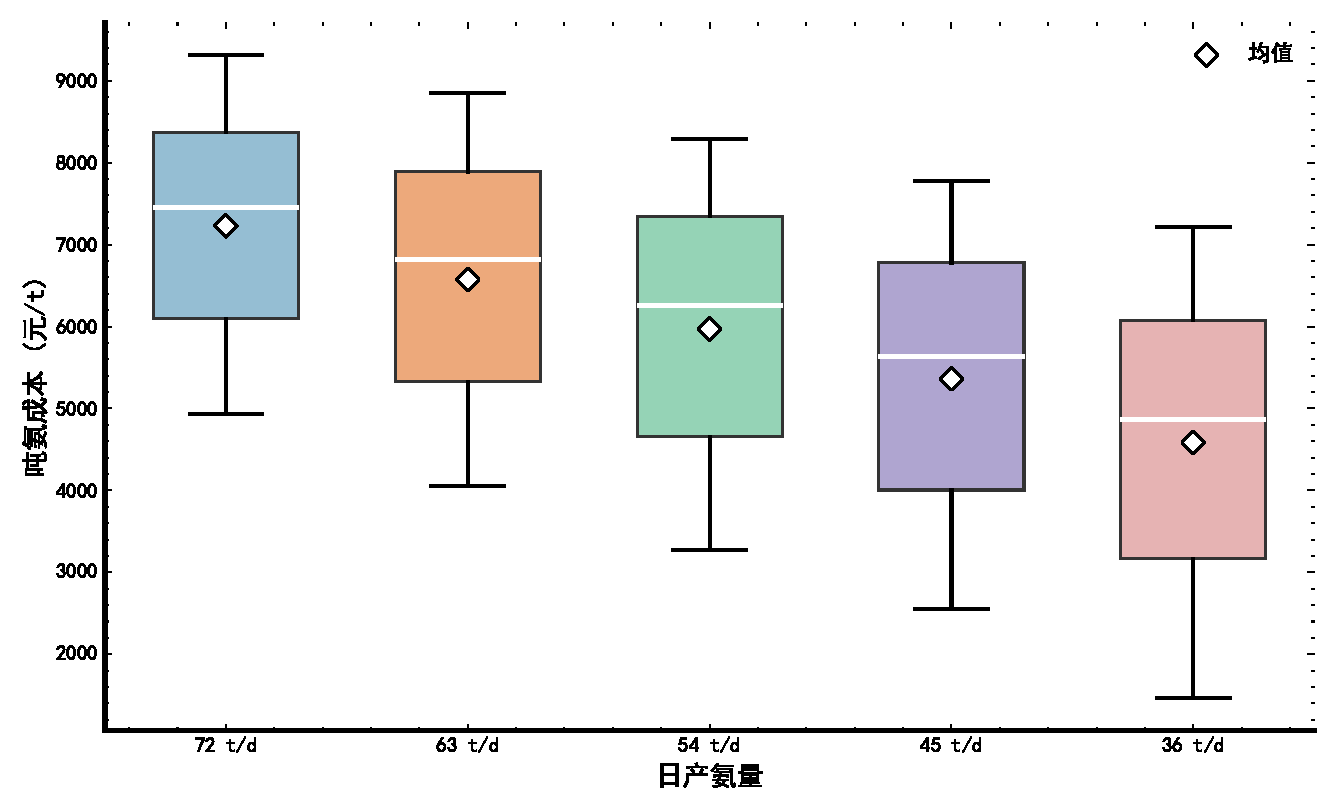
\includegraphics[width=0.85\textwidth]{../figures/fig_q2_24scenes_cost.pdf}
\caption{24种风光场景下各产量吨氨成本分布箱线图}\label{fig:q2_24scenes_cost}
\end{figure}

各产量下的年均吨氨成本和成本范围如表\ref{tab:q2_annual}所示。全年最优产量为36吨/日，年均吨氨成本4585.15元/吨，但成本波动范围最大（1461.72--7216.48元/吨），反映了低产量方案对风光资源条件的高度敏感性。高产量方案（72吨/日）虽然年均成本最高（7228.33元/吨），但成本波动相对较小，运行稳定性更好。

\begin{table}[H]
\centering
\caption{24种场景全年分析结果}\label{tab:q2_annual}
\begin{tabular}{cccccc}
\toprule
产量(吨/日) & 均值成本 & 最小成本 & 最大成本 & 全满足(场景数) & 全不满足 \\
\midrule
72 & 7228.33 & 4935.96 & 9318.91 & 18 & 0 \\
63 & 6575.46 & 4054.66 & 8848.86 & 14 & 0 \\
54 & 5970.54 & 3272.91 & 8289.00 & 14 & 1 \\
45 & 5363.38 & 2548.43 & 7777.19 & 1 & 4 \\
36 & 4585.15 & 1461.72 & 7216.48 & 0 & 3 \\
\bottomrule
\end{tabular}
\end{table}

\subsubsection{绿电指标统计}

假设每种风光场景代表15天，24种场景覆盖全年360天。以产量36吨/日为例，全年绿电指标统计为：全满足0天、部分满足315天、全不满足45天。绿电指标满足情况的统计如图\ref{fig:q2_indicator_stats}所示。

\begin{figure}[H]
\centering
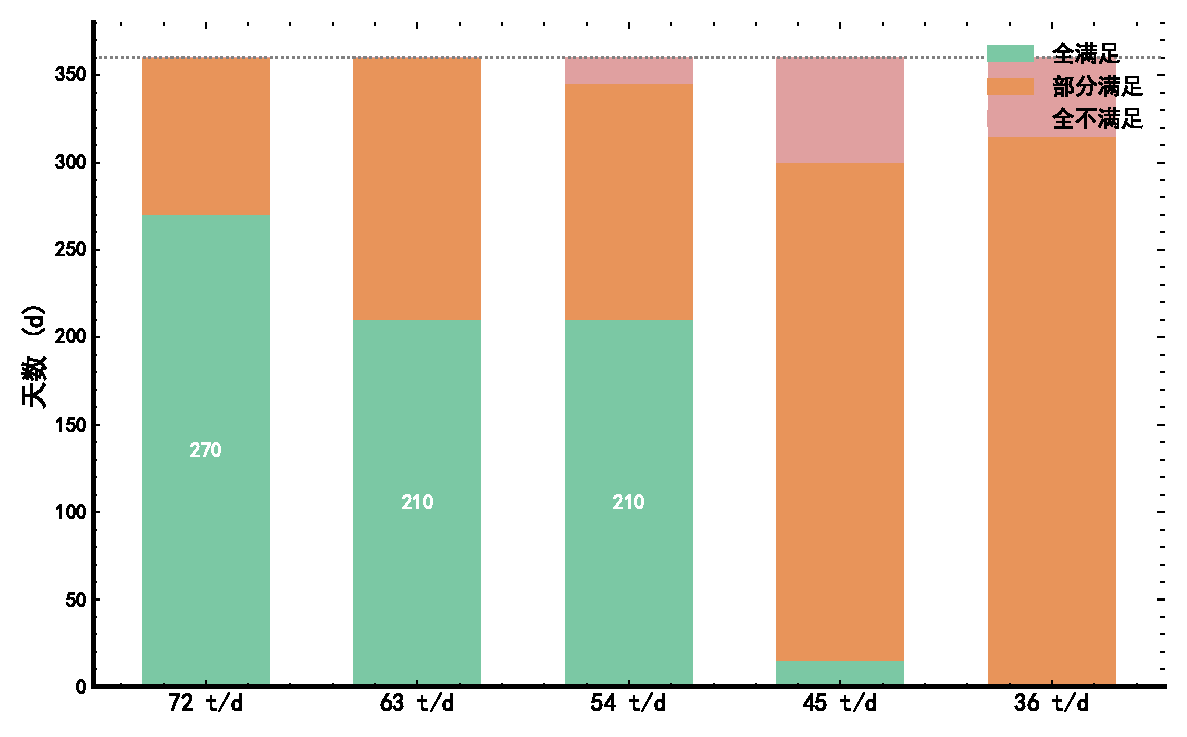
\includegraphics[width=0.85\textwidth]{../figures/fig_q2_indicator_stats.pdf}
\caption{全年绿电直连指标满足情况统计}\label{fig:q2_indicator_stats}
\end{figure}

高产量方案（72吨/日）的绿电指标表现最好，全满足天数达270天（18个场景$\times$15天），这是因为高产量意味着更多的电力被就地消纳，减少了上网电量。低产量方案虽然经济性更优，但绿电合规性显著恶化，存在成本与合规之间的权衡关系。

\subsubsection{全年吨氨成本分布}

全年吨氨成本分布曲线如图\ref{fig:q2_annual_cost}所示，该曲线反映了在离散调节模式下，不同风光资源条件对生产成本的影响。成本分布呈现右偏特征，低风光场景对应的高成本尾部较长，表明极端不利天气条件下的经济性风险较大。

\begin{figure}[H]
\centering
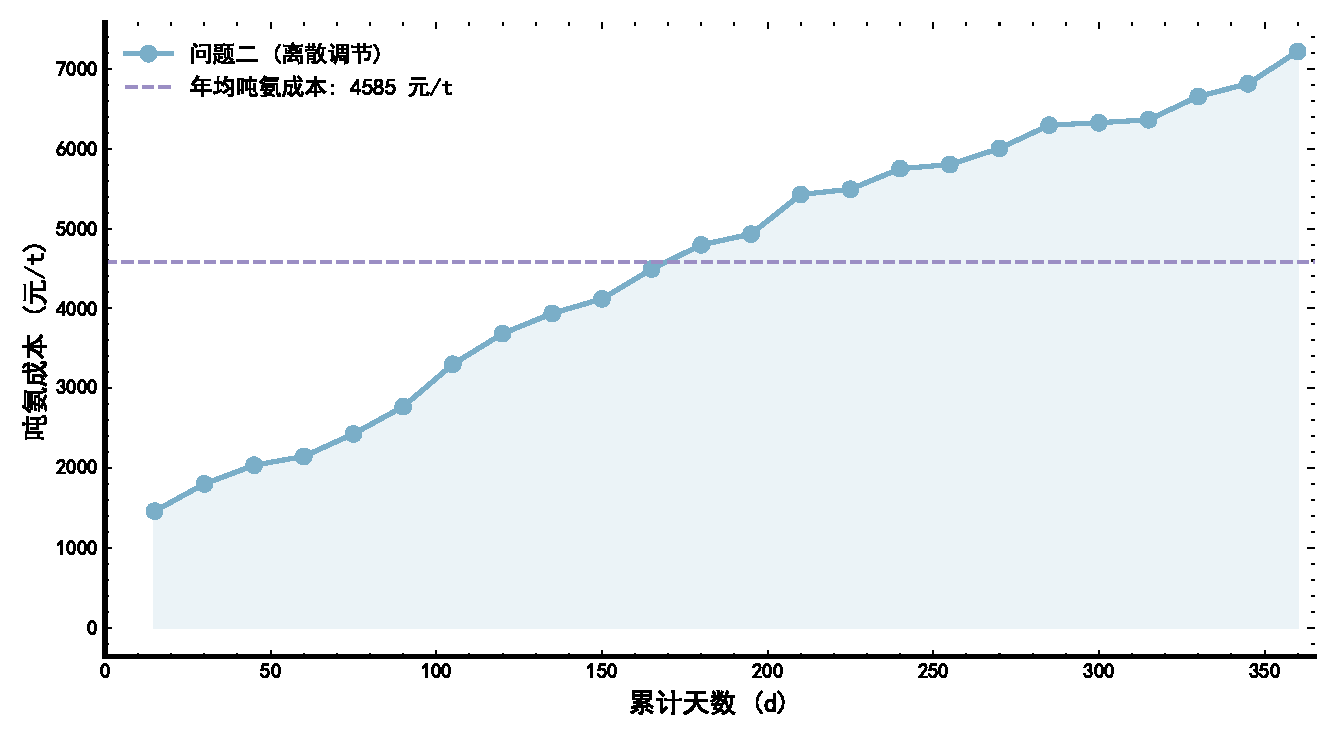
\includegraphics[width=0.85\textwidth]{../figures/fig_q2_annual_cost.pdf}
\caption{全年吨氨成本分布曲线（离散调节，36吨/日）}\label{fig:q2_annual_cost}
\end{figure}
